\chapter{Zusammenführung und Vergleich}
\label{chap:vergleich}
Um die mit beiden Ansätzen gefundenen Cluster weiter zu untermauern, wurden die zu jedem Cluster gehörenden Benutzer*innen verglichen, um zu untersuchen, ob es möglich ist, Cluster aus dem Retweet-Netzwerk-Ansatz Cluster aus dem Sprach-Clustering-Ansatz zuzuordnen.
Um die Beziehung zu veranschaulichen, wurde ein Sankey-Diagramm erstellt, das links die Netzwerkcluster, rechts die Sprachcluster und Benutzer, die Teil von zwei Clustern sind, als grauen Fluss darstellt. Benutzer aus den Netzwerkclustern, die keinem Sprachcluster angehören, fließen nach "undefined".
\begin{figure}[h!]
	\centering
	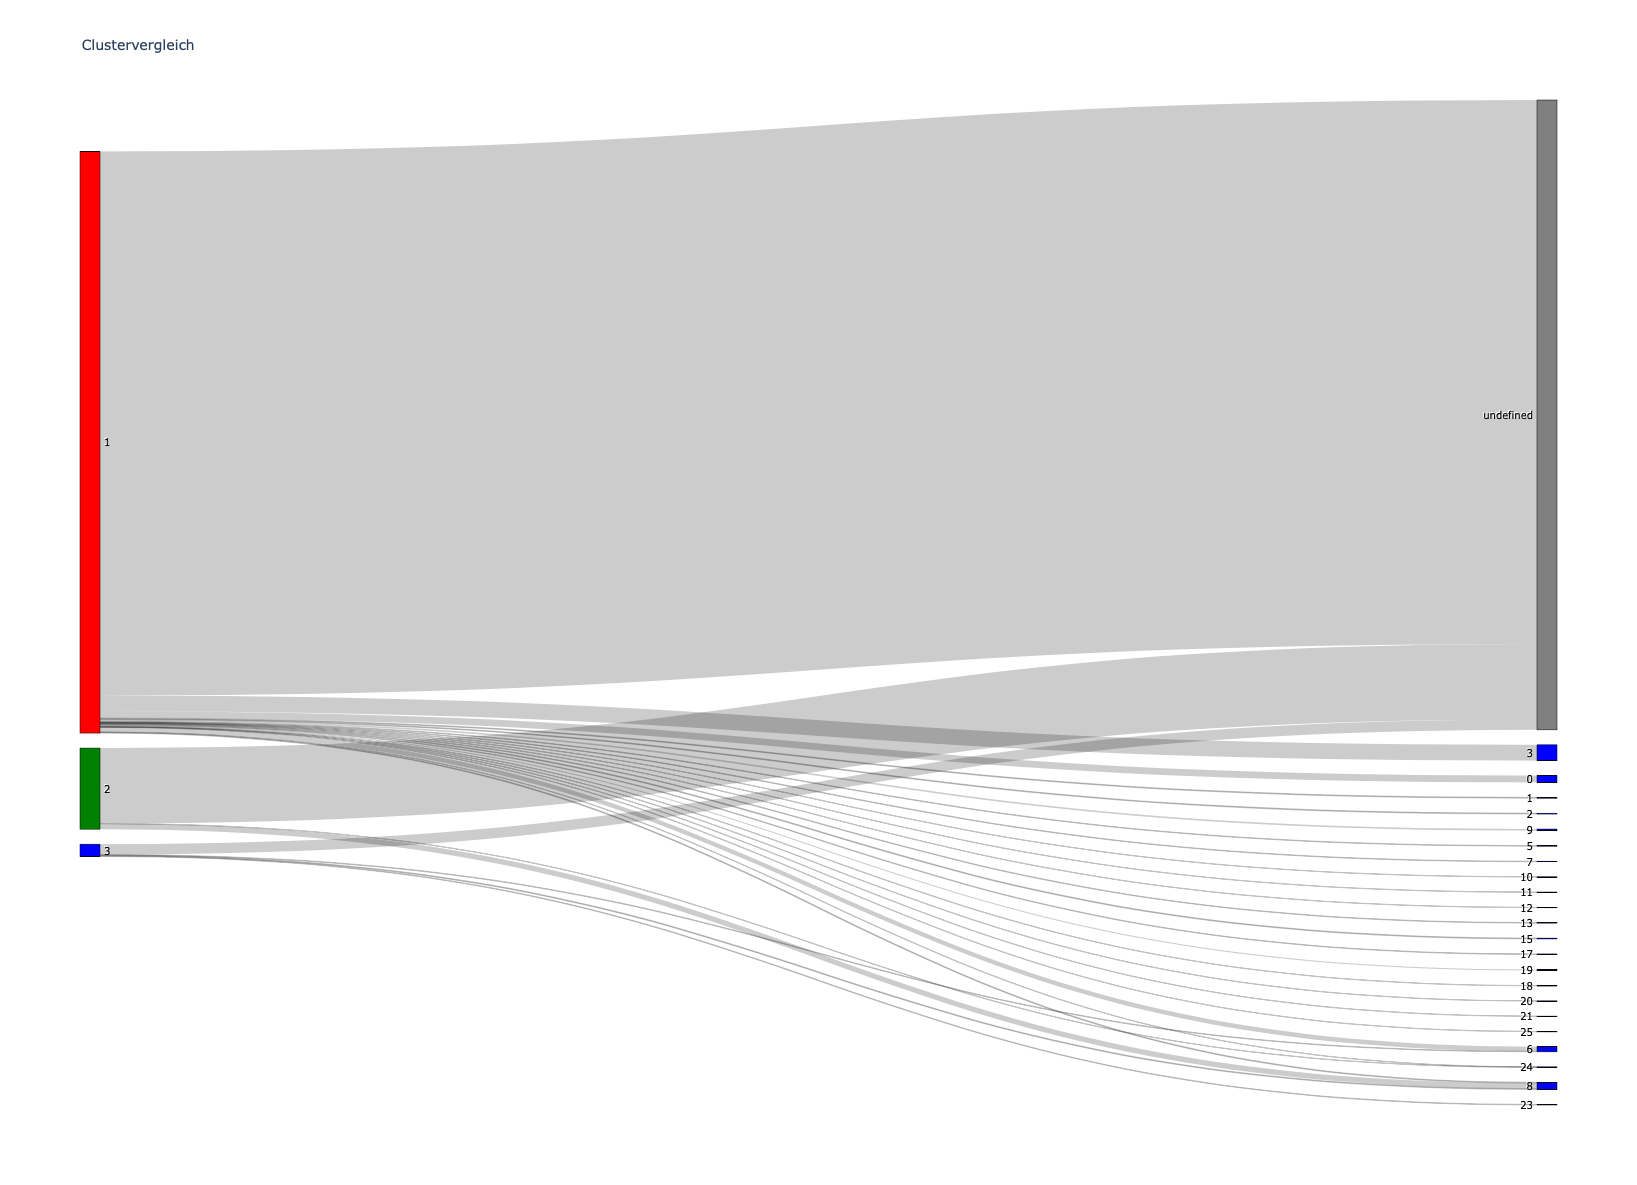
\includegraphics[width=0.7\linewidth]{images/VergleichUndefined}
	\caption{Benutzerassoziationen zwischen Clustern der beiden Ansätze}
	\label{fig:vergleichundefined}
\end{figure}
Mehr als 50\% der Benutzer aus den Netzwerkclustern wurden nicht im Sprachansatz geclustert (auch vice versa).
Dies kann durch die Schritte in beiden Ansätzen erklärt werden die das Filtern von Benutzern beinhalten:
Der Rohdatensatz enthält 260.954 Benutzer.
\section{Filterschritte im Netzwerkansatz}
\begin{itemize}
	\item Nur Benutzer*innen werden berücksichtigt, die retweeten: 37\% (966.322) der Benutzer*innen werden herausgefiltert
	\item Nur Benutzern*innen werden berücksichtigt, die Influencer retweeten: 57\% der Benutzer, die retweeten (94.730), werden herausgefiltert
	\item Anwenden eines Schwellenwerts auf Superuser-Verbindungen:\\
	Da einige Superuser gelöscht werden, wenn alle ihre Verbindungen unter dem Schwellenwert liegen, werden ihre zugehörigen Benutzer*innen aus dem Cluster gefiltert. 96\% der Nutzer, die Influencer retweeten (67.119), werden herausgefiltert
\end{itemize}
\section{Filterschritte im Sprachansatz}
\begin{itemize}
	\item Es werden nur die Hashtags verwendet, deren Anzahl zwischen dem 97\% und 99,98\% Quantil der Häufigkeitsverteilung liegt: 98\% (404.905) der Hashtags werden herausgefiltert
	\item Nur die Benutzer, die diese Hashtags mehr als 6 Mal innerhalb des Monats verwendet haben, werden beibehalten: 99,5\% (238.717) aller Benutzer werden herausgefiltert
\end{itemize}
Da beide Ansätze den Datensatz nach unterschiedlichen Merkmalen filtern, ist die durchschnittliche Anzahl der Nutzer, die in den Ergebnissen für beide Ansätze vorhanden sind, sehr gering  Ein identisches Filterverfahren für beide Ansätze würde dieses Problem lösen.